\chapter{Samples} \label{chap:ex}

Neste capítulo exemplifica-se como inserir alguns ambientes (enumeração, tabela, figura).

\begin{enumerate}
	\item Resistência\index{Resistência} -- É um elemento passivo que dissipa energia sob a forma térmica;
	\item Condensador\index{Condensador} -- É um elemento que armazena energia num campo eléctrico.
\end{enumerate}

A Tabela \ref{tab:001} contém o código de cores das resistências\footnote{Apenas código para primeira e segunda cor. Não inclui tolerância nem factor multiplicativo. Apenas código para primeira e segunda cor. Não inclui tolerância nem factor multiplicativo. Apenas código para primeira e segunda cor. Não inclui tolerância nem factor multiplicativo}.

\begin{table}[h!]
\caption{Correspondência entre as cores das riscas das resistências e o seu valor óhmico.}
	\centering
		\begin{tabular}{|c|c|}
		\hline
			\textbf{Cor} & \textbf{Valor} \cr
			\hline
			Preto & 0 \cr
			\hline
			Castanho & 1 \cr
			\hline
			Vermelho & 2 \cr
			\hline
			Laranja & 3 \cr
			\hline
			Amarelo & 4 \cr
			\hline
			Verde & 5 \cr
			\hline
			Azul & 6 \cr
			\hline
			Violeta & 7 \cr
			\hline
			Cinzento & 8 \cr
			\hline
			Branco & 9 \cr
			\hline
		\end{tabular}
	\label{tab:001}
\end{table}

Considere-se o circuito da Figura \ref{fig:ohm}.

\begin{figure}[h]
	\centering
		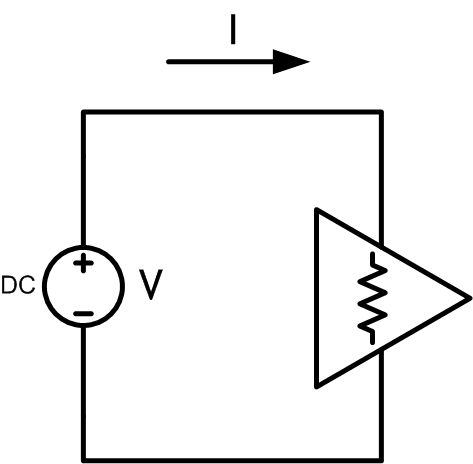
\includegraphics[height=3cm]{leiOhm}
	\caption{Circuito básico com uma fonte de tensão contínua (V) e uma resistência atravessada por uma corrente I.}
	\label{fig:ohm}
\end{figure}

Pode-se calcular a corrente que circula na resistência através da equação \ref{for:ohm}, denominada de Lei de Ohm\index{Lei de Ohm}.


\begin{equation}\label{for:ohm}
	I=\frac{V}{R}
\end{equation}

O texto pode vir em \textbf{negrito} ou em \textit{itálico} ou \textbf{\textit{ambos}}.

O Algoritmo \ref{alg1} serve de base para o nosso sistema de controlo do semáforo da igreja.
\begin{algorithm}
	\caption{Pseudo código para o semáforo.}
	\label{alg1}
	\begin{algorithmic}
		\STATE Início
		\FOR{todas as luzes}
			\IF{sem corrente}
				\STATE informar de avaria
			\ELSE
				\STATE luz ok
			\ENDIF 
		\ENDFOR
		
		\LOOP
			\STATE accionar verde no semáforo principal
			\STATE aguardar por sinal dos sensores de posição
			\IF{carro no sensor}
				\STATE mudar para vermelho semáforo principal
			\ENDIF
		\ENDLOOP
		\STATE \textbf{until} interruptor de manutenção activado
	\end{algorithmic}
\end{algorithm}

